\documentclass[]{article}
\usepackage{lmodern}
\usepackage{amssymb,amsmath}
\usepackage{ifxetex,ifluatex}
\usepackage{fixltx2e} % provides \textsubscript
\ifnum 0\ifxetex 1\fi\ifluatex 1\fi=0 % if pdftex
  \usepackage[T1]{fontenc}
  \usepackage[utf8]{inputenc}
\else % if luatex or xelatex
  \ifxetex
    \usepackage{mathspec}
    \usepackage{xltxtra,xunicode}
  \else
    \usepackage{fontspec}
  \fi
  \defaultfontfeatures{Mapping=tex-text,Scale=MatchLowercase}
  \newcommand{\euro}{€}
\fi
% use upquote if available, for straight quotes in verbatim environments
\IfFileExists{upquote.sty}{\usepackage{upquote}}{}
% use microtype if available
\IfFileExists{microtype.sty}{%
\usepackage{microtype}
\UseMicrotypeSet[protrusion]{basicmath} % disable protrusion for tt fonts
}{}
\usepackage[margin=1in]{geometry}
\usepackage{color}
\usepackage{fancyvrb}
\newcommand{\VerbBar}{|}
\newcommand{\VERB}{\Verb[commandchars=\\\{\}]}
\DefineVerbatimEnvironment{Highlighting}{Verbatim}{commandchars=\\\{\}}
% Add ',fontsize=\small' for more characters per line
\usepackage{framed}
\definecolor{shadecolor}{RGB}{248,248,248}
\newenvironment{Shaded}{\begin{snugshade}}{\end{snugshade}}
\newcommand{\KeywordTok}[1]{\textcolor[rgb]{0.13,0.29,0.53}{\textbf{{#1}}}}
\newcommand{\DataTypeTok}[1]{\textcolor[rgb]{0.13,0.29,0.53}{{#1}}}
\newcommand{\DecValTok}[1]{\textcolor[rgb]{0.00,0.00,0.81}{{#1}}}
\newcommand{\BaseNTok}[1]{\textcolor[rgb]{0.00,0.00,0.81}{{#1}}}
\newcommand{\FloatTok}[1]{\textcolor[rgb]{0.00,0.00,0.81}{{#1}}}
\newcommand{\CharTok}[1]{\textcolor[rgb]{0.31,0.60,0.02}{{#1}}}
\newcommand{\StringTok}[1]{\textcolor[rgb]{0.31,0.60,0.02}{{#1}}}
\newcommand{\CommentTok}[1]{\textcolor[rgb]{0.56,0.35,0.01}{\textit{{#1}}}}
\newcommand{\OtherTok}[1]{\textcolor[rgb]{0.56,0.35,0.01}{{#1}}}
\newcommand{\AlertTok}[1]{\textcolor[rgb]{0.94,0.16,0.16}{{#1}}}
\newcommand{\FunctionTok}[1]{\textcolor[rgb]{0.00,0.00,0.00}{{#1}}}
\newcommand{\RegionMarkerTok}[1]{{#1}}
\newcommand{\ErrorTok}[1]{\textbf{{#1}}}
\newcommand{\NormalTok}[1]{{#1}}
\usepackage{graphicx}
\makeatletter
\def\maxwidth{\ifdim\Gin@nat@width>\linewidth\linewidth\else\Gin@nat@width\fi}
\def\maxheight{\ifdim\Gin@nat@height>\textheight\textheight\else\Gin@nat@height\fi}
\makeatother
% Scale images if necessary, so that they will not overflow the page
% margins by default, and it is still possible to overwrite the defaults
% using explicit options in \includegraphics[width, height, ...]{}
\setkeys{Gin}{width=\maxwidth,height=\maxheight,keepaspectratio}
\ifxetex
  \usepackage[setpagesize=false, % page size defined by xetex
              unicode=false, % unicode breaks when used with xetex
              xetex]{hyperref}
\else
  \usepackage[unicode=true]{hyperref}
\fi
\hypersetup{breaklinks=true,
            bookmarks=true,
            pdfauthor={},
            pdftitle={},
            colorlinks=true,
            citecolor=blue,
            urlcolor=blue,
            linkcolor=magenta,
            pdfborder={0 0 0}}
\urlstyle{same}  % don't use monospace font for urls
\setlength{\parindent}{0pt}
\setlength{\parskip}{6pt plus 2pt minus 1pt}
\setlength{\emergencystretch}{3em}  % prevent overfull lines
\setcounter{secnumdepth}{0}

%%% Use protect on footnotes to avoid problems with footnotes in titles
\let\rmarkdownfootnote\footnote%
\def\footnote{\protect\rmarkdownfootnote}

%%% Change title format to be more compact
\usepackage{titling}

% Create subtitle command for use in maketitle
\newcommand{\subtitle}[1]{
  \posttitle{
    \begin{center}\large#1\end{center}
    }
}

\setlength{\droptitle}{-2em}
  \title{}
  \pretitle{\vspace{\droptitle}}
  \posttitle{}
  \author{}
  \preauthor{}\postauthor{}
  \date{}
  \predate{}\postdate{}



\begin{document}

\maketitle


\section{Statistical Inference}\label{statistical-inference}

\subsubsection{Course Project 2:
CP2\_template}\label{course-project-2-cp2ux5ftemplate}

\subsubsection{Introduction}\label{introduction}

This document presents the results of the Course Project for the
Coursera course: Statistical Inference. This assessment makes use of
statistical techniques in order to explore the relationship between the
tooth size of guinea pigs and vitamin dosage levels.

\subsubsection{Data}\label{data}

This assignment makes use of the `toothgrowth' data set. The data set
consists of measurements of length of guinea pigs teeth. It also states
that there are two delivery methods of Vitamin C, orange juice (OJ) and
ascorbic acid (VC). They were administered with three dose levels of
0.5, 1, and 2 mg.

\begin{itemize}
\itemsep1pt\parskip0pt\parsep0pt
\item
  Dataset:
  \href{https://stat.ethz.ch/R-manual/R-devel/library/datasets/html/ToothGrowth.html}{toothgrowth
  data}
\end{itemize}

It consists of 60 observations on 3 variables.

\subsubsection{1. Load Packages/Data}\label{load-packagesdata}

\begin{Shaded}
\begin{Highlighting}[]
\NormalTok{for (package in }\KeywordTok{c}\NormalTok{(}\StringTok{'ggplot2'}\NormalTok{, }\StringTok{'plyr'}\NormalTok{)) \{}
 
    \NormalTok{if (!}\KeywordTok{require}\NormalTok{(package, }\DataTypeTok{character.only =} \OtherTok{TRUE}\NormalTok{, }\DataTypeTok{quietly =} \OtherTok{FALSE}\NormalTok{)) \{}
        \KeywordTok{install.packages}\NormalTok{(package)}
        \KeywordTok{library}\NormalTok{(package, }\DataTypeTok{character.only =} \OtherTok{TRUE}\NormalTok{)}
    \NormalTok{\}}
\NormalTok{\}}

\KeywordTok{data}\NormalTok{(ToothGrowth)}
\NormalTok{data_tooth <-}\StringTok{ }\NormalTok{ToothGrowth}
\end{Highlighting}
\end{Shaded}

\subsubsection{2. Exploratory Data
Analysis}\label{exploratory-data-analysis}

Show data summary:

\begin{Shaded}
\begin{Highlighting}[]
\KeywordTok{summary}\NormalTok{(data_tooth)}
\end{Highlighting}
\end{Shaded}

\begin{verbatim}
##       len        supp         dose      
##  Min.   : 4.20   OJ:30   Min.   :0.500  
##  1st Qu.:13.07   VC:30   1st Qu.:0.500  
##  Median :19.25           Median :1.000  
##  Mean   :18.81           Mean   :1.167  
##  3rd Qu.:25.27           3rd Qu.:2.000  
##  Max.   :33.90           Max.   :2.000
\end{verbatim}

Check recorded tooth legnth against dosage level:

\begin{Shaded}
\begin{Highlighting}[]
\KeywordTok{ggplot}\NormalTok{(data_tooth, }\KeywordTok{aes}\NormalTok{(}\DataTypeTok{x =} \NormalTok{dose, }\DataTypeTok{y =} \NormalTok{len)) +}\StringTok{ }
\StringTok{  }\KeywordTok{geom_point}\NormalTok{(}\DataTypeTok{size =} \DecValTok{3}\NormalTok{, }\DataTypeTok{colour =} \StringTok{"blue"}\NormalTok{) +}
\StringTok{  }\KeywordTok{ggtitle}\NormalTok{(}\StringTok{'Figure 1: Avg. Tooth Length vs. Dosage Level'}\NormalTok{)}
\end{Highlighting}
\end{Shaded}

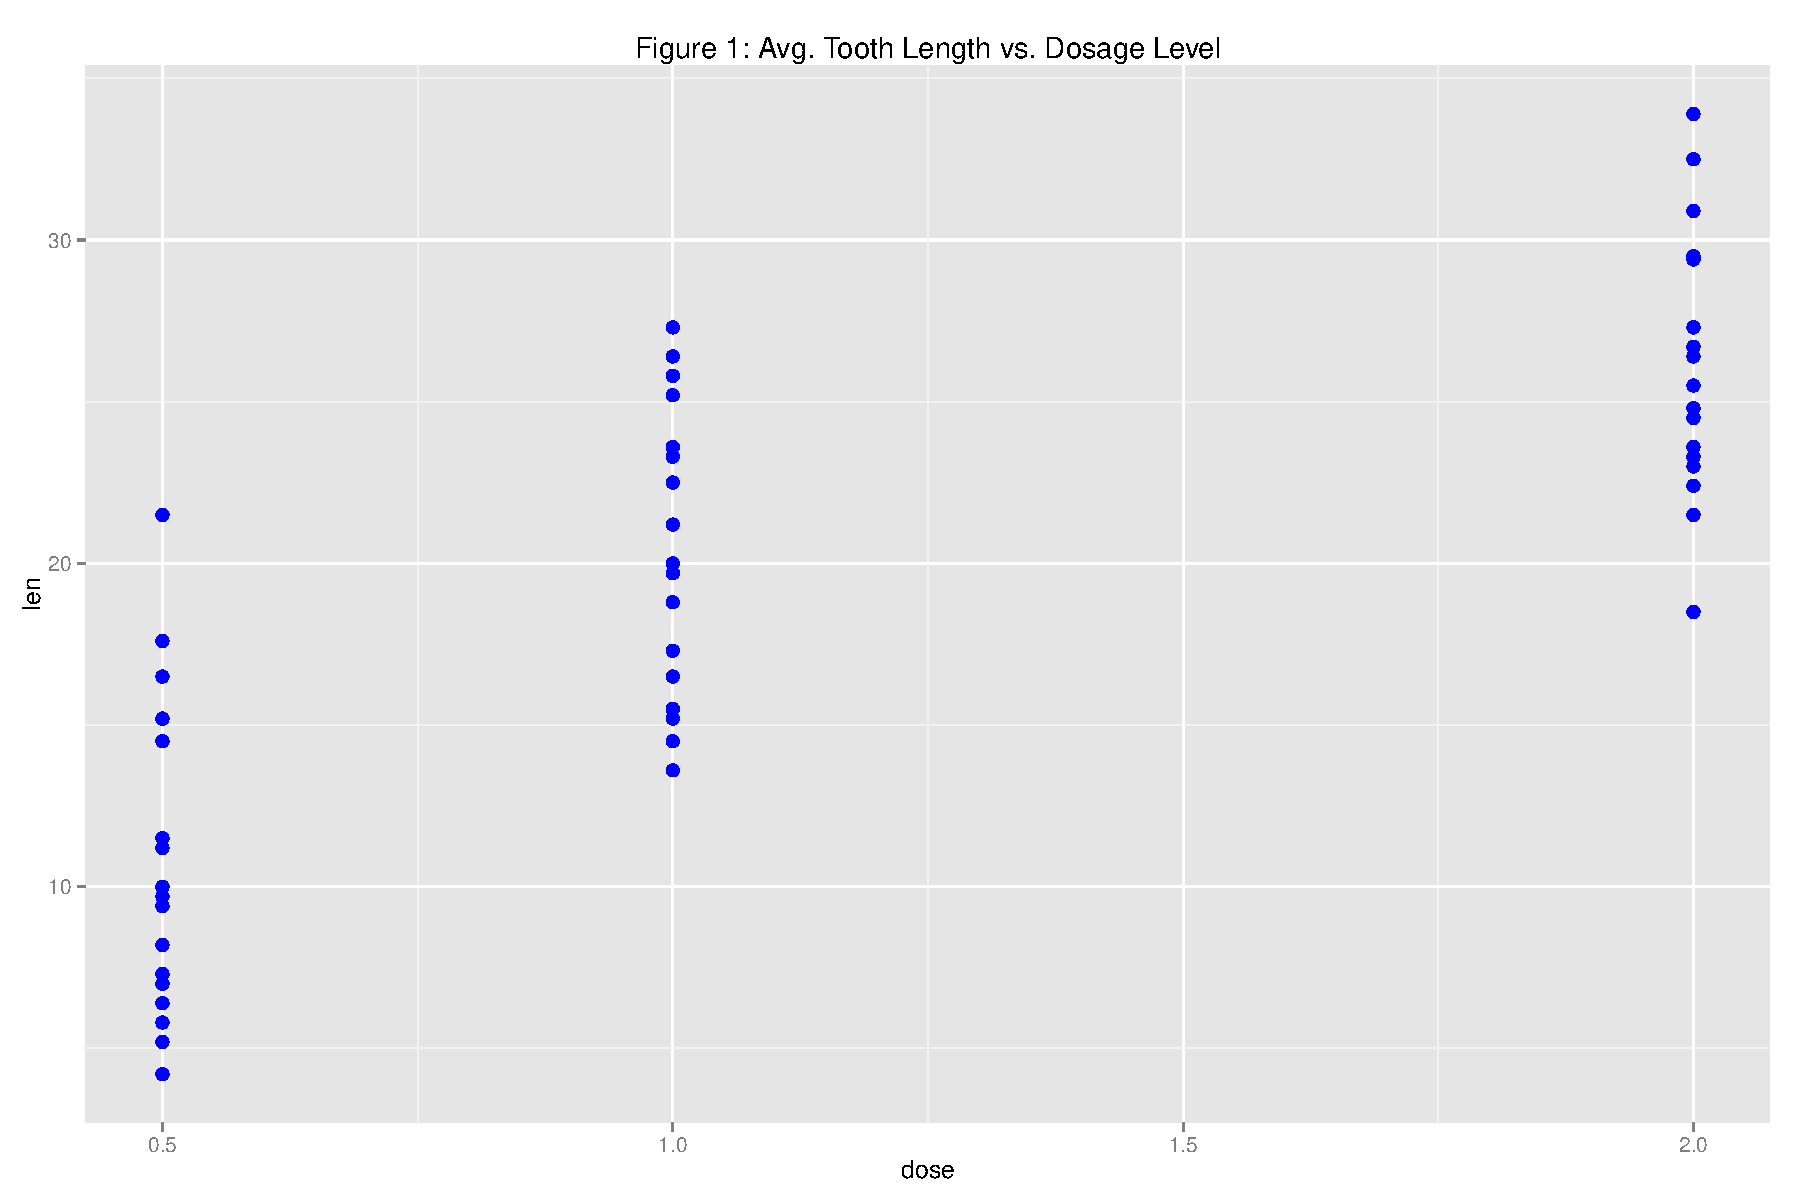
\includegraphics{figure/unnamed-chunk-3-1.pdf} The plot suggests a
positive correlation between recorded tooth length and dosage level.

\subsubsection{3. Confidence Interval
Analysis}\label{confidence-interval-analysis}

Use confidence intervals and hypothesis tests to compare tooth growth by
supplement type and dose level:

\begin{Shaded}
\begin{Highlighting}[]
\KeywordTok{ddply}\NormalTok{(data_tooth, dose ~}\StringTok{ }\NormalTok{supp, function(x) }
  \KeywordTok{c}\NormalTok{(}\DataTypeTok{mean =} \KeywordTok{mean}\NormalTok{(x$len),}
  \DataTypeTok{sd =} \KeywordTok{sd}\NormalTok{(x$len),}
  \DataTypeTok{conf.int =} \KeywordTok{t.test}\NormalTok{(x$len)$conf.int))}
\end{Highlighting}
\end{Shaded}

\begin{verbatim}
##   dose supp  mean       sd conf.int1 conf.int2
## 1  0.5   OJ 13.23 4.459709 10.039717 16.420283
## 2  0.5   VC  7.98 2.746634  6.015176  9.944824
## 3  1.0   OJ 22.70 3.910953 19.902273 25.497727
## 4  1.0   VC 16.77 2.515309 14.970657 18.569343
## 5  2.0   OJ 26.06 2.655058 24.160686 27.959314
## 6  2.0   VC 26.14 4.797731 22.707910 29.572090
\end{verbatim}

It is observed that the `VC' intervals are pairwise disjoint (95\%
confidence level). As such, tooth length means are taken as distinct and
a positive correlation between recorded tooth length and dosage level is
again observed.

The `OJ' intervals however, are overlapped between the 1.0 and 2.0
dosage levels. Therefore, explicit tests for these dosages are
performed:

\begin{Shaded}
\begin{Highlighting}[]
\NormalTok{val_ttest1 <-}\StringTok{ }\KeywordTok{t.test}\NormalTok{(len ~}\StringTok{ }\NormalTok{dose, }\DataTypeTok{paired =} \OtherTok{FALSE}\NormalTok{, }\DataTypeTok{var.equal =} \OtherTok{TRUE}\NormalTok{, }\DataTypeTok{data =} \KeywordTok{subset}\NormalTok{(data_tooth, dose %in%}\StringTok{ }\KeywordTok{c}\NormalTok{(}\FloatTok{1.0}\NormalTok{, }\FloatTok{2.0}\NormalTok{) &}\StringTok{ }\NormalTok{supp ==}\StringTok{ 'OJ'}\NormalTok{))}
\NormalTok{val_ttest2 <-}\StringTok{ }\KeywordTok{t.test}\NormalTok{(len ~}\StringTok{ }\NormalTok{supp, }\DataTypeTok{paired =} \OtherTok{FALSE}\NormalTok{, }\DataTypeTok{var.equal =} \OtherTok{FALSE}\NormalTok{, }\DataTypeTok{data =} \KeywordTok{subset}\NormalTok{(data_tooth, dose ==}\StringTok{ }\FloatTok{2.0}\NormalTok{))}

\KeywordTok{data.frame}\NormalTok{(}\DataTypeTok{row.names =} \KeywordTok{c}\NormalTok{(}\StringTok{"'1.0 OJ dose' vs '2.0 OJ dose'"}\NormalTok{, }\StringTok{"'2.0 OJ dose' vs '2.0 VC dose'"}\NormalTok{),}
  \StringTok{"p-value"} \NormalTok{=}\StringTok{ }\KeywordTok{c}\NormalTok{(val_ttest1$p.value, val_ttest2$p.value),}
  \StringTok{"Conf-Low"} \NormalTok{=}\StringTok{ }\KeywordTok{c}\NormalTok{(val_ttest1$conf[}\DecValTok{1}\NormalTok{], val_ttest2$conf[}\DecValTok{1}\NormalTok{]),}
  \StringTok{"Conf-High"} \NormalTok{=}\StringTok{ }\KeywordTok{c}\NormalTok{(val_ttest1$conf[}\DecValTok{2}\NormalTok{], val_ttest2$conf[}\DecValTok{2}\NormalTok{]))}
\end{Highlighting}
\end{Shaded}

\begin{verbatim}
##                                  p.value  Conf.Low  Conf.High
## '1.0 OJ dose' vs '2.0 OJ dose' 0.0373628 -6.500502 -0.2194983
## '2.0 OJ dose' vs '2.0 VC dose' 0.9638516 -3.798070  3.6380705
\end{verbatim}

For `OJ', it is observed that the mean length for a 1.0 dosage level is
greater than the mean length for a 2.0 dosage level (p-value = 0.037).
For the 2.0 dosage level however, it is observed that the difference
between type of supplement is insignificant (p-vale = 0.964).

\subsubsection{4. Conclusion}\label{conclusion}

Analysis has shown positive correlation between dosage levels and the
tooth size of guinea pigs. For lower level dosages (0.5mg and 1.0mg),
Orange Juice supplement has an advantage over the Vitamin C supplement.
However for the 2.0mg dosage level there is no significant difference
between the type of supplement used.

\end{document}
